The algorithm implementation was tested on a simulated set of events.
For this purpose 500\,000 $(a,b)$ events were Monte-Carlo generated according to the function
\begin{equation}
\label{eq:simul}
1 + x_1a + x_2a^2 + x_3b + x_4b^2
\end{equation}
with the parameters
\{$x_1 = 0.5$, $x_2 = 0.3$, $x_3 = 0.8$, $x_4 = 0.1$\}.
Then the same equation \eqref{eq:simul} was fitted to them using an event-by-event log.\ likelihood method with constraints
\begin{equation}
\label{eq:simul:constr}
x_1^2 + x_1x_4 - x_4^2 = 0.29,~x_2^2/x_3 = 0.1125.
\end{equation}

% Results:
% \begin{figure}[htbp]\centering
% 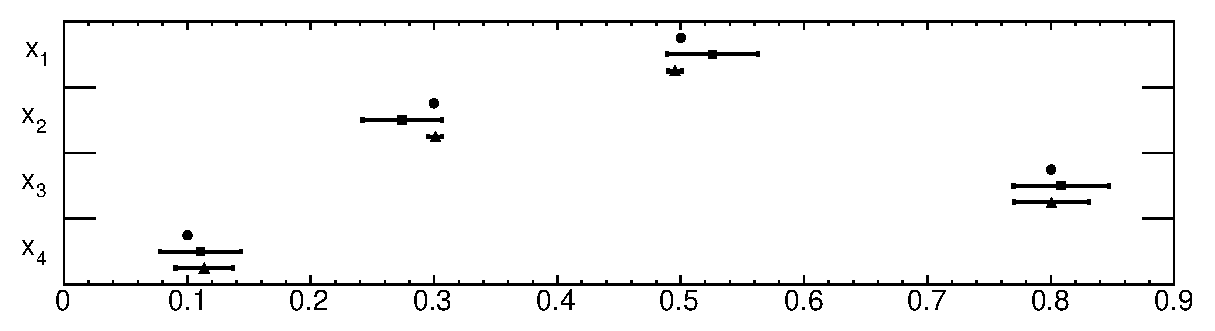
\includegraphics[width=1\textwidth]{pics/drawToyBW.eps}
% \caption{
% The parameter values obtained by fitting the set of events generated according to the equation \eqref{eq:simul}.
% Circles correspond to the original values used in the simulation, squares show the results provided by the fit without constraints, triangles come from the fit with constraints \eqref{eq:simul:constr}.
% }
% \label{toy_errs}
% \end{figure}

\begin{table}[htbp]
\caption{
Parameter values obtained by fitting the set of events generated according to equation \eqref{eq:simul}, with their errors.
}
\label{tab:1}
\begin{tabular*}{1\textwidth}{@{\hspace{2em}}c@{\extracolsep{\fill}}ccc@{\hspace{2em}}}\hline\hline
Parameter & True values & Unconstrained fit & Constrained fit \\\hline
$x_1$ & $0.5$ & $0.526 \pm 0.037$ & $0.496 \pm 0.006$ \\
$x_2$ & $0.3$ & $0.274 \pm 0.032$ & $0.301 \pm 0.006$ \\
$x_3$ & $0.8$ & $0.808 \pm 0.039$ & $0.801 \pm 0.030$ \\
$x_4$ & $0.1$ & $0.111 \pm 0.033$ & $0.114 \pm 0.023$ \\\hline\hline
\end{tabular*}
\end{table}

The results of the fit are presented in
% fig.~\ref{toy_errs} and
table~\ref{tab:1}. They show that constraints could lead to significant improvement in fit precision, that is particularly pronounced in the present case for the parameters $x_2$ and $x_3$.
